% vim: ft=tex fdm=marker et sts=2 sw=2
%! TEX program = pdfLaTeX

\documentclass[10pt,oneside,article]{memoir}

\usepackage[utf8]{inputenc}
\usepackage[T1]{fontenc}

\usepackage{tikz,lipsum}
% \usepackage[draft]{emem}
\usepackage{emem}
\usepackage{fourierx}

\title{Title of the Article\thanks{A test {\LaTeX} file for testing \texttt{emem.sty}.}}
\author{%
  A.~Author\thanks{Adress of A.~Author; \email{a.author@mail.zz}} \and%
  B.~Author\thanks{Adress of B.~Author} \and%
  C.~Author\thanks{Adress of C.~Author}%
}
\date{1 January 1970}

\begin{document}

\maketitle

\begin{abstract}
  \lipsum[1]
\end{abstract}

\section{Section Title}
\lipsum[1]

\subsection{Subsection Title}
\lipsum[2]

\subsubsection{Subsubsection Title}
\lipsum[3]

\paragraph{Paragraph}
\lipsum[4]


\makeatletter
  \def\Inter@scale{0.8}
\makeatother
{\fontseries{semibold}\fontfamily{Inter-LF}\selectfont Hello world}

\section{Figures and figure captions}

Captions of figures look a bit different\ldots
\begin{figure}[h]
  \begin{center}
    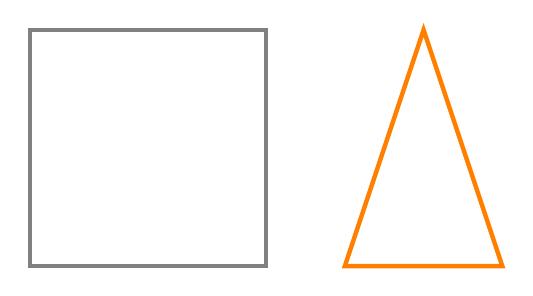
\begin{tikzpicture}
      \draw[gray, ultra thick] (0,0) rectangle (3,3);
      \draw[orange, ultra thick] (4,0) -- (5,3) -- (6,0) -- cycle;
    \end{tikzpicture}
  \end{center}
  \caption{The caption of the figure is set in sans font (if the \texttt{sanscaptions} option is given) in ``small'' font size.  Mathematics is typed like this: $E^2=p^2c^2 + m^2c^4$.}
\end{figure}

\section{Mathematics}

\subsection{Operators}

Examples of new math operators:
\begin{equation}
  \trace{A}\quad \Trace{A}\quad \erf{x}\quad \Residue{f}\quad \corank{A}\quad \rank{B}
\end{equation}

\subsection{Bold letters}

Check when Computer Modern, or its variant, is used. \textbf{This is TEXT bold}.  Math version:
\begin{equation}
  \mathbf{ABCDEFGHIJKLMNOPQRSTUVWXYZ}\quad \mathbf{abcdefghijklmnopqrstuvwxyz}
\end{equation}

\end{document}
